\chapter{BLAST-TNG Target selection: B-field Morphology in Nearby External Galaxies}\label{galaxies}

Our understanding of the Milky Way's ISM is greatly augmented by observations of nearby galaxies. Results from the BLAST 2006 balloon flight (2006) revealed that over half of the FIR background is associated with galaxies at z $\geq$ 1.2 \citep{blast2006}. These galaxies are spatially unresolved, although estimates of their global properties may be improved by factoring in inferences made from observations of resolved galaxies. \citet{blastresolved} attempted to constrain estimates of the star formation rate (SFR) in the aforementioned population of unresolved galaxies by placing an upper limit on the amount of active galactic nuclei (AGN) driven dust heating in a sample of six nearby (d $\leq{20}$~Mpc) AGN\@. This `AGN fraction' is the observed ratio of core-flux to extended-flux. Using total intensity measurements for six nearby galaxies surveyed by BLAST 2006, the authors were able to derive the dust mass absorption coefficient, and found that the sample of nearby galaxies contains a higher dust mass than would be predicted based on observations of unresolved sub-mm galaxies.

As a sub-mm imaging polarimeter with spatial resolution of $\approx$30$\arcsec$ at 250~$\upmu$m, BLAST-TNG will be capable of measuring dozens of \gls{Bpos} pseudovectors for galaxies at distances of around 10~Mpc (a physical scale of $\sim$1~kpc). This mapping resolution is comparable to that which is commonly achieved by single-dish radio observatories operating at wavelengths of a few centimeters. The resulting maps of \gls{Bpos} can be compared to existing observations of \gls{Bpos} in these targets in order to gain a better understanding of the three-dimensional structure of the large-scale B-field. The total intensity maps will be useful for further analysis of global dust properties within external galaxies.

In the following sections, we describe the selection of five nearby galaxies which will be observed during the 2019/2020 BLAST-TNG flight from McMurdo, Station, Antarctica. They are organized as follows:

\begin{itemize}[nosep]
  \item Section~\ref{previous obs} describes some of the key observational inferences which have been made concerning B-fields in external galaxies.
  \item Section~\ref{target selection} summarizes the galaxy targets which have been selected for observation by BLAST-TNG\@.
  \item In Section~\ref{mapping speed} we present estimates of the mapping time required for BLAST-TNG to measure sufficient SNRs on the polarization fraction of each target galaxy.
\end{itemize}

\section{Summary of Previous Observations}\label{previous obs}

Observations of extragalactic B-fields aim to address the fundamental questions of how the original fields were seeded, amplified, and shaped into their presently observed morphologies. In addition, open questions remain concerning the degree to which large-scale B-fields influence the evolution of galaxies through the role they play in energetic processes, and in governing SFRs\@. On galaxy scales, the energy density of B-fields is generally assumed to be in equipartition with that of cosmic rays. In most galaxies, including the Milky Way, the average equipartition B-field strength is of $\mathcal{O}$(10)~$\upmu$G. The field strength is observed to be weaker in radio-quiet galaxies, and stronger in galaxies containing active star formation \citep{beck2016magnetic}. B-fields are physically important on a wide range of scales, from the intergalactic to the interstellar medium (IGM, ISM). They are responsible for channeling cosmic rays throughout (and between) galaxies, and play a role in star formation within molecular clouds (MCs). However, astronomical B-fields are difficult to measure. To date, the best tracer of B-fields is polarized emission in wavebands ranging from the radio to the optical. Observations of Zeeman splitting, radio synchrotron emission, Faraday rotation and differential dust extinction (in the O/NIR or sub-mm/mm-wave bands) can reveal the strength of one or more B-field components. However, Zeeman splitting is the only known measurement technique which can directly probe the strength of the field (for \gls{Blos}).

\subsection{Radio Measurements of External Galaxies}
Over the past few decades, several surveys of polarized synchrotron emission in nearby galaxies have been undertaken in order to map the large-scale fields in a variety of galaxy types, including spirals, ellipticals, dwarf irregulars and interacting pairs \citep{van2015magnetic}. Synchrotron measurements yield estimates of \gls{Bpos}. These measurements can be combined with Faraday rotation measures (RM), which trace \gls{Bpos}, in order to glean information about the three-dimensional structure of the fields. The large-scale B-field geometries of a few dozen galaxies have been studied in detail (see, e.g, \citet{sofue1985large,beck2005magnetic,beck2016magnetic}). While many of the observed extragalactic B-field configurations can be understood as being the result of small and mean-scale dynamo mechanisms (see Section~\ref{dynamo}), some morphologies defy classification by existing theories (e.g, M81 \citet{beck2006origin}).

These radio observations have led to several key inferences. Perhaps the most wide-reaching inference is the discovery that the integrated radio continuum emission at centimeter wavelengths is strongly correlated with the degree of sub-mm/FIR emission in galaxies with active star formation (the radio-FIR correlation) (\citet{de1985astronomy,beck2008measuring}). Because most of the radio emission at centimeter wavelengths is from non-thermal synchrotron radiation, the synchrotron emission (which traces \gls{Bpos}) can be used to estimate the SFR\@.

The polarized synchrotron emission, which traces the ordered component of galactic B-fields, has been observed to be strongest in the inter-arm regions of spiral galaxies \citep{beck2016magnetic}. In these galaxies the toroidal field (in the plane of the disk) often forms arms which fill the inter-arm regions. These magnetic arms follow the optically bright spiral arms, but occasionally deviate from the large-scale spiral pattern formed by the gas and dust. Within the material arms, the B-field is turbulent and irregular. The poloidal field (the field which occupies the halo), which is most easily observed in galaxies with high inclination angles (close to edge-on), frequently forms an \textit{X} shape, which is thought to be generated by bipolar outflows of ionized material \citep{ferriere2014analytical}. Figure~\ref{fig:m51} shows a map of \gls{Bpos} pseudovectors in M51, obtained from VLA and Effelsberg measurements at 6~cm, overplotted with an optical image from the Hubble Space Telescope (HST) \citep{fletcher2011magnetic}. The inter-arm B-field tracks the spiral pattern of the optical arms, but extends well beyond the visible extent of the gas and dust.

\begin{figure}[!htbp]
\centering
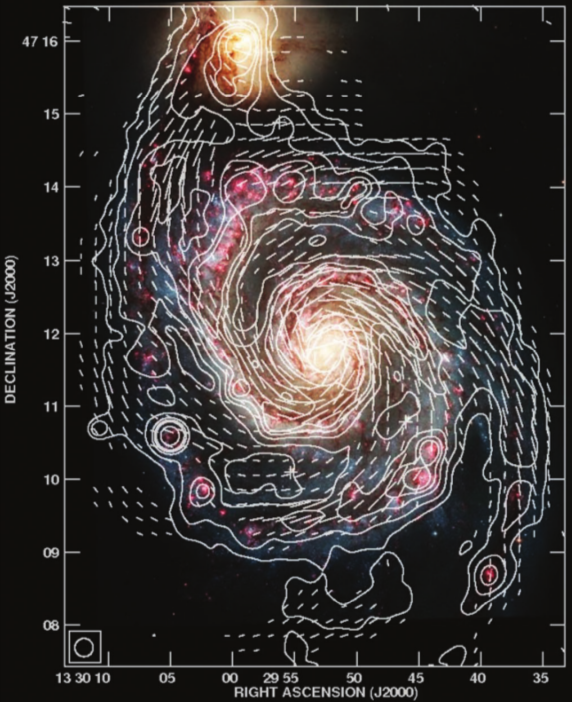
\includegraphics[width=0.7\textwidth]{figures/galaxies/m51}
\caption[A composite radio image of the large-scale B-field in M51.]{The large-scale B-field in M51 (\gls{Phi} pseudovectors), revealed by VLA and Effelsberg measurements taken at 6~cm, with a spatial resolution of 6$\arcsec$. The background optical image is from HST \citep{fletcher2011magnetic}.}
\label{fig:m51}
\end{figure}

\subsection{The Modal Structure of Large-Scale Magnetic Fields}\label{dynamo}

Although the mechanism by which the primordial seed fields were created (magnetogenesis) is not well understood (see, e.g., \citet{kandus2011primordial}), the theory which describes how galactic seed fields are amplified to their observed equipartition values of $\mathcal{O}$(10)~$\upmu$G has for the most part been well matched by observations \citep{beck2006origin}. The seed fields are thought to have been amplified over several million years by a small-scale dynamo. This dynamo is generated by turbulence created by supernovae and density wave shocks within spiral arms, which shear and compress the B-field. These processes result in a turbulent field geometry, having no regular direction on small scales. The field is then ordered and sustained on large-scales over several billion years by the $\alpha-\Omega$ mechanism, where $\alpha$ refers to the Coriolis Effect, and $\Omega$ refers to differential rotation. The mechanism is described by the mean-field dynamo equation:

\begin{equation}\label{eq:dynamo}
\frac{\partial \textbf{B}}{\partial t} = \nabla \times (v \times \textbf{B}) + \nabla \times \alpha \textbf{B} + \eta \nabla^{2} \textbf{B}
\end{equation}

where $\nabla \times (v \times \textbf{B})$ represents field amplification, $\nabla \times \alpha \textbf{B}$ is a gain term from the Coriolis effect, and $\eta \nabla^{2} \textbf{B}$ is a loss term which accounts for the friction of diffusion between ionized and neutral gas. For the dynamo to work, gas flows associated with supernova remnants in a disk expand and rise, causing B-field loops to form via the Coriolis effect. In turn, the field loops generate ion flows that produce new, regular fields loops in a plane perpendicular to the disk. The solutions to the mean-field dynamo equation are azimuthal Fourier modes: $\boldsymbol{B} = \sum_{m} \beta_{m}\cos(m\phi - \beta)$, where $\beta$ is a phase and $\phi$ is the azimuthal angle in the plane of the disk \citep{sofue1985large}.

The two lowest toroidal modes, axisymmetric ($m$ = 0) and bisymmetric ($m$ = 1), are accompanied by even (quadrupolar) and odd (dipolar) parity poloidal modes. The lower order modes are easier to excite and amplify than the higher order modes, and most well studied spiral galaxies exhibit a superposition of the two, with axisymmetric being the more dominant mode. Combined radio measurements of polarized synchrotron emission and Faraday RMs can be used to partially decompose the modes \citep{beck2008measuring}.

\subsection{Measurements of Polarized Submillimeter Emission in External Galaxies}

Measurements of the sub-mm polarization fraction $p$ in external galaxies can advance theories of magnetic dust-grain alignment. They have also been used to characterize the role that external galaxies may play as a CMB foreground \citep{seiffert2006upper}. In contrast to the growing catalog of radio observations of external galaxies, there is a paucity of complementary observations of polarized emission at sub-mm wavelengths. Part of this discrepancy is explained by the relatively small number of sub-mm telescopes which possess the spatial resolution of large, single-dish radio observatories. Consequently, more attempts have been made to map \gls{Bpos} on large-scales using differential dust extinction in the O/NIR (see, e.g., \citet{fendt1998spiral}).

The first sub-mm mapping of \gls{Bpos} in another galaxy was reported for M82, a nearby starbust galaxy \citep{greaves2000magnetic}. This observation was taken at 850~$\upmu$m, with the SCUBA instrument (Submillimeter Common User Bolometer Array) on the James Clerk Maxwell Telescope (JCMT). The spatial resolution of the map is $\sim$15$\arcsec$ ($\sim$280~pc). These observations revealed that M82 possesses a large-scale toroidal field which is ordered on scales of at least that of the map resolution. A poloidal field surrounding the nucleus was also noted. Surprisingly, the orientation of the fields as traced by the polarized sub-mm dust emission were found to be unaligned with the galactic plane.

A more recent sub-mm observation of M82 was taken at 53~$\upmu$m and 154~$\upmu$m with the HAWC+ instrument (High-resolution Airborne Wideband Camera-plus) on the Stratospheric Observatory for Infrared Astronomy (SOFIA) \citep{jones2019sofia}. These observations resolved poalrized emission from thermal dust on scales of $\sim$90~pc. A LIC map of \gls{Bpos} at 154~$\upmu$m is shown in Figure~\ref{fig:m82 lic}. The LIC map of M82 shows that \gls{Bpos} has a vertical orientation in the inner region of the galaxy, and a planar orientation in the outer regions of the disk. The inner, vertically oriented field corresponds to the region where a starburst is occurring. The authors of the study note that the high amount of beam-averaging prohibits the application of DCFM to these maps.

\begin{figure}[!htbp]
\centering
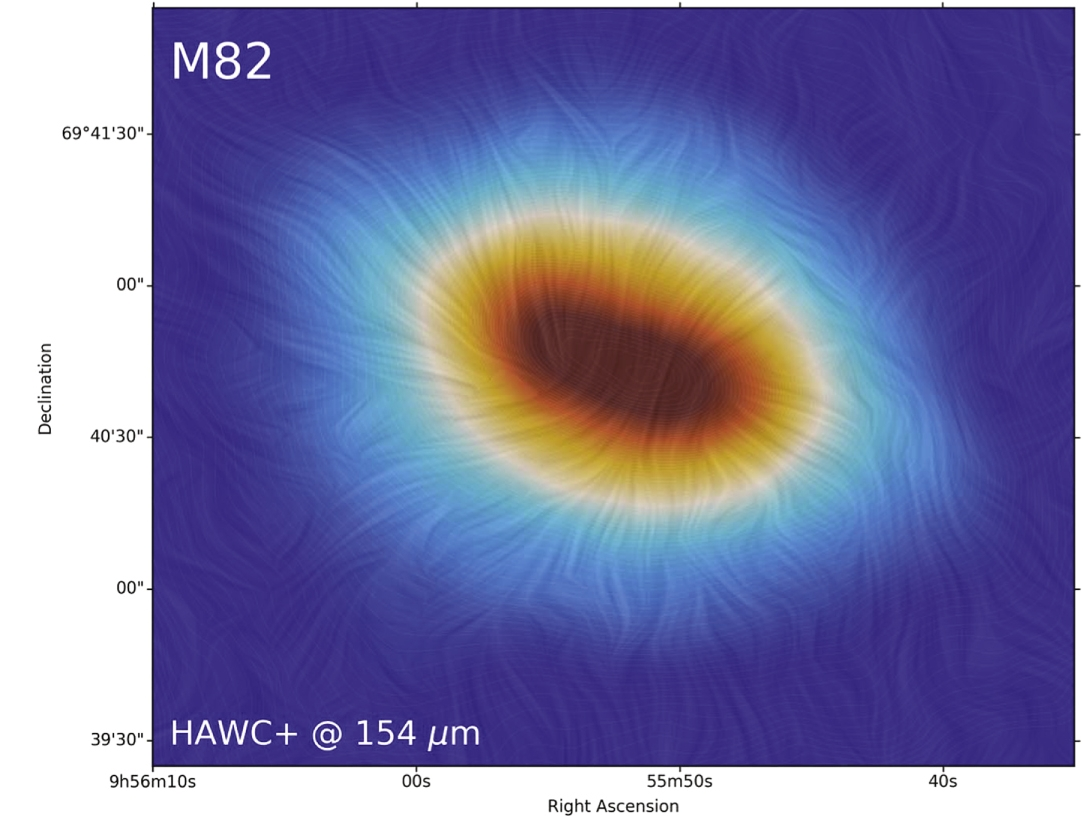
\includegraphics[width=0.7\textwidth]{figures/galaxies/m82_lic_cropped}
\caption[A LIC map of M82, taken with the \macrocapwrap{154~$\upmu$m} channel of the HAWC+ instrument on SOFIA.]{A LIC map of M82, taken with the 154~$\upmu$m channel of the HAWC+ instrument on SOFIA \citep{jones2019sofia}.}
\label{fig:m82 lic}
\end{figure}

\section{BLAST-TNG External Galaxy Targets}\label{target selection}

The five external galaxies which have been selected for observation by BLAST-TNG were chosen based on several criteria. The primary constraint comes from the telescope's visibility, which will change throughout the flight as the stratospheric circumpolar vortex winds carry the telescope around the Antarctic continent. During the flight, the telescope's latitude might change by up to 10~degrees. The telescope can move in elevation between 22 and 50 degrees, with limits on azimuth imposed by the position of the sun (it should be kept out of view of the primary mirror). Roughly, observable targets must fall within the range of 5 to 18 hours of RA, and -62 to -23 degrees of declination.

The second selection criterion is that the galaxies should be bright enough for BLAST-TNG to be able to measure an SNR on the polarization-fraction of $\gtrsim$3 (see Section~\ref{mapping speed}). Galaxies which satisfy the first two criteria are deemed more desirable if previous observations of their B-fields exist, particularly those based on measurements of polarized synchrotron emission or Faraday RMs.

\subsection{Target List}\label{targ list}

The five galaxy targets, along with their sky coordinates, distance, resolvable spatial scale at 250~$\upmu$m and type are listed in Table~\ref{table:gal targs}.

%\begin{threeparttable}[!htbp]
\begin{table}[!htbp]
\centering
\begin{tabular}{@{}llllll@{}}
\dtoprule{}
Object & RA (J2000) & DEC (J2000) & \begin{tabular}[c]{@{}l@{}} Distance \\ (kpc) \end{tabular} & \begin{tabular}[c]{@{}l@{}}Scale$_{250}$ \\ (kpc) \end{tabular} & Type  \\ \midrule
NGC 4945 & 13:05:27.279 & -49:28:04.44 & 3,900 & 0.57 & SB(s)cd \\
ESO 97-G13 & 14:13:09.906 & -65:20:20.47 & 4,200 & 0.61 & SA(s)b \\
% NGC 5068 & 13:18:54.807 & -21:02:20.76 & 6,075 & 0.82 & SB(s)d \\
NGC 3621 & 11:18:16.5     & -32:48:51  &  6,700 & 0.97 & SA(s)d \\
NGC M83 & 13:37:00.919 & -29:51:56.74 & 8,900 & 1.29 & SA(s)ab \\
NGC 1808 & 05:07:42.343 & -37:30:46.98 & 10,900 & 1.59 & (R$^{\prime}$)SAB(s)b \\
% NGC 2997 & 09:45:38.793 & -31:11:27.92 & 15,900 & 2.31 & SA(s)c\\
\dbottomrule{}
\\
\end{tabular}
%\begin{tablenotes}
%    \item[1] Laboca.\\
%  \end{tablenotes}
\caption[A summary of five nearby galaxy targets selected for observation by BLAST-TNG.]{A summary of the five nearby galaxy targets selected for observation by BLAST-TNG, listed in order of their distance.}
\label{table:gal targs}
\end{table}

\textit{NGC 4945}: NGC 4945 is an edge-on, Seyfert~2 (Sy2) type spiral galaxy which is otherwise thought to be similar to the Milky Way \citep{spoon2000mid}. To date, no radio halo has been detected in NGC 4945 \citep{elmouttie1997radio}.

\vspace{5mm}

\textit{ESO 97-G13}: ESO 97-G13 (AKA the Circinus Galaxy) is a near edge-on Sy2 galaxy located close to the Galactic plane. Its bipolar radio lobes have been mapped at centimeter wavelengths using ATCA \citep{elmouttie1998radio}. The radio lobes are associated with ionized plumes being ejected from the AGN. The B-field in the radio lobes is observed to be aligned with the plume axis.

\vspace{5mm}

\textit{NGC 3621}: NGC 3621 is a near edge-on spiral field galaxy. There is no evidence for a bulge in the galaxy's center, but it is thought to be a Sy2 type \citep{barth2008dynamical}. The HI continuum was recently mapped at 6$\arcsec$ resolution using the Very Large Array (VLA), as part of the THINGS survey of nearby galaxies \citep{walter2008things}.

\vspace{5mm}

\textit{M83}: M83 (NGC 5236, AKA the Southern Pinwheel Galaxy) is a nearby, nearly face-on grand-design spiral galaxy of the starburst variety. It is located near the dwarf galaxy, NGC 5253, which also hosts a high level of active star formation. M83 has been observed in a wide range of wavebands, and the large-scale structure of its B-field has been mapped in polarized synchrotron emission (\citet{sukumar1989large,frick2016magnetic}). The B-field is of the inter-arm spiral type. The authors of \citet{frick2016magnetic} compared the radio observations of M83 to sub-mm total intensity maps, and found that the orientation of one of the main B-field arms is misaligned with its corresponding gaseous arms.

%\textit{NGC 2997}: NGC 2997 is a face-on unbarred spiral galaxy, whose scale B-field has previously been mapped using Faraday RMs (\citet{han1999magnetic}). The RM map revealed an anomalous field reversal between the disk and central region of the galaxy. An unusually high degree of radio polarization  ($\sim$25\%) has been reported along the inner edges of the galaxy's spiral arms (\citet{beck2016magnetic}).

\vspace{5mm}

\textit{NGC 1808}: NGC 1808 is a Sy2 type galaxy which was mapped by BLAST 2006 \citep{blastresolved}. Its large-scale B-field has been mapped in optical polarization, which revealed a coherent toroidal magnetic spiral, with no visible poloidal component \citep{scarrott1993imaging}. \citet{siebenmorgen2001infrared} detected polarized emission at 170~$\upmu$m along four sightlines through the galaxy, and found that the polarization angles differ significantly from those measured from nonthermal polarized radio emission \citep{siebenmorgen2001infrared}.

%\vspace{5mm}

%\textit{NGC 5068}: NGC 5068 is a nearly face-on, barred spiral galaxy. It has been found to be radio-weak, with no halo polarization detected to date (\citet{beck2005magnetic}).

%IRAS
%\citet{neugebauer1984infrared}
%PHANGS
%\citet{leroy2016portrait}
%KINGFISH
%\citet{dale2012herschel}

\subsection{Required Observing Times}\label{mapping speed}

In this section we present estimates of the minimum integration times which are required to make 3-$\sigma$ measurements of $p$ for each of the galaxy targets described in Section~\ref{targ list}\footnote{A detailed description of the methods presented here can be found at: \url{https://sites.northwestern.edu/blast/}}.

The minimum beam-averaged intensity ($\mathrm{MJy/sr}$) which is required to achieve 1-$\sigma$ error bars on $p$ of $\sigma_{p}$, over a map of area $A_{\mathrm{map}}$ (deg$^{2}$), in $t$ hours, is:

\begin{equation}\label{eq:Ireq}
  I_{\mathrm{req}} = I_{\mathrm{ref}} \left( \frac{A_{\mathrm{map}}}{1 \text{ deg}^{2}}  \right)^{1/2} \left( \frac{5 \text{ hr}}{t} \right)^{1/2} \left( \frac{0.005}{\sigma_{p} } \right) \qquad \left[ \mathrm{MJy/sr} \right]
\end{equation}

where $I_{\mathrm{ref}}$ ($\mathrm{MJy/sr}$) is the intensity which is required to measure $\sigma_{p}$ = 0.5\%, after a 5~hr integration over a 1~deg$^{2}$ map (see Table~\ref{table:map speed}). The required observing time to achieve 1-$\sigma$ error bars on $p$ of $\sigma_{p}$ over a map of area $A_{\mathrm{map}}$ (deg$^{2}$), for a source with intensity $I_{\mathrm{req}}$, is:

\begin{equation}\label{eq:treq}
  t_{\mathrm{req}} = t_{\mathrm{ref}} \left( \frac{A_{\mathrm{map}}}{1 \text{ deg}^{2}}  \right) \left( \frac{0.005}{\sigma_{p} } \right)^{2} \left(  \frac{100 \textrm{ MJy/sr}}{I_{\mathrm{req}}} \right)^{2} \qquad \left[ \mathrm{hr} \right]
\end{equation}

where $t_{\mathrm{ref}}$ is the time required to obtain $\sigma_{p} = 0.5$\% for a source with $I = 100$~MJy/sr (see Table~\ref{table:map speed}).

\begin{table}[!htbp]
\centering
\begin{tabular}{@{}llll@{}}
\dtoprule{}
 & 250~$\upmu$m & 350~$\upmu$m & 500~$\upmu$m \\ \midrule
$I_{\mathrm{ref}}$ ($\mathrm{MJy/sr}$) & 188.7 & 113.7 & 42.4 \\
$t_{\mathrm{ref}}$ ($\mathrm{hr}$) & 17.8 & 6.4 & 0.9 \\
Beam FWHM ($\arcsec$) & 30 & 41 & 59 \\ \dbottomrule{}
\\
\end{tabular}
\caption[Reference values for BLAST-TNG mapping calculation.]{Reference values for calculating the required target intensity $I_{\mathrm{req}}$ and observation time $t_{\mathrm{req}}$ to achieve a desired maximum uncertainty on the polarization-fraction $\sigma_{p}$. The reference intensity $I_{\mathrm{ref}}$ (MJy/sr) is the beam-averaged source intensity which is required to measure $\sigma_{p}$ = 0.5\%, after a 5~hr integration over a 1~deg$^{2}$ map. The reference integration time $t_{\mathrm{ref}}$ (hr) is the time required to obtain $\sigma_{p} = 0.5$\% for a source with an intensity of 100~MJy/sr. Table values are taken from \url{https://sites.northwestern.edu/blast/}. The beam FWHM for each observation band (in arcsec) is listed in the third row.}
\label{table:map speed}
\end{table}

The smallest maps that BLAST-TNG will make will be $\sim$0.5~deg$^{2}$. Because the galaxy targets fit into this area, their map size will be uniformly $\sim$0.5 deg$^{2}$. Table~\ref{table:treq} lists the required integration time $t_{\mathrm{req}}$, in hours, needed to achieve $\sigma_{p} = 0.5$\% over the region of each galaxy which is visible in the the Herschel 250~$\upmu$m total intensity maps. Three of the targets require at least 7~hr of integration time. The brightest targets, NGC 4945 and ESO 97-G13, require at least 3~hr.

\begin{table}[!htbp]
\centering
\begin{tabular}{@{}lllll@{}}
\dtoprule{}
Object & A$_{\mathrm{map}}$ (deg$^{2}$) & $\sigma_{p}$ (\%) & t$_{\mathrm{req}}$ (hr) & I$_{250}$ center (MJy/sr) \\ \midrule
NGC 4945 & 0.5 & 0.5 & 3 & 10,000 \\
ESO 97-G13 & 0.5 & 0.5 & 3 & 3,600 \\
NGC 3621 & 0.5 & 0.5 & 7 & 150 \\
M83 & 0.5 & 0.5 & 7 & 1,000 \\
NGC 1808 & 0.5 & 0.5 & 7 & 2,500 \\ \dbottomrule{}
\\
\end{tabular}
\caption[Key mapping parameters for the BLAST-TNG external galaxy targets.]{Map area $A_{\mathrm{map}}$, 1-$\sigma$ polarization-fraction $\sigma_{p}$, integration time $t_{\mathrm{req}}$, and central beam-averaged intensity from Herschel 250~$\upmu$m maps for each BLAST-TNG galaxy target}
\label{table:treq}
\end{table}

Figures~\ref{fig:ngc4945} to~\ref{fig:ngc1808} show the Herschel 250~$\upmu$m maps for each galaxy target. The colorscales are (left frame) $t_{\mathrm{req}}$ in hours, and (right frame) intensity in $\mathrm{MJy/sr}$.

\begin{figure}[!htbp]
\centering
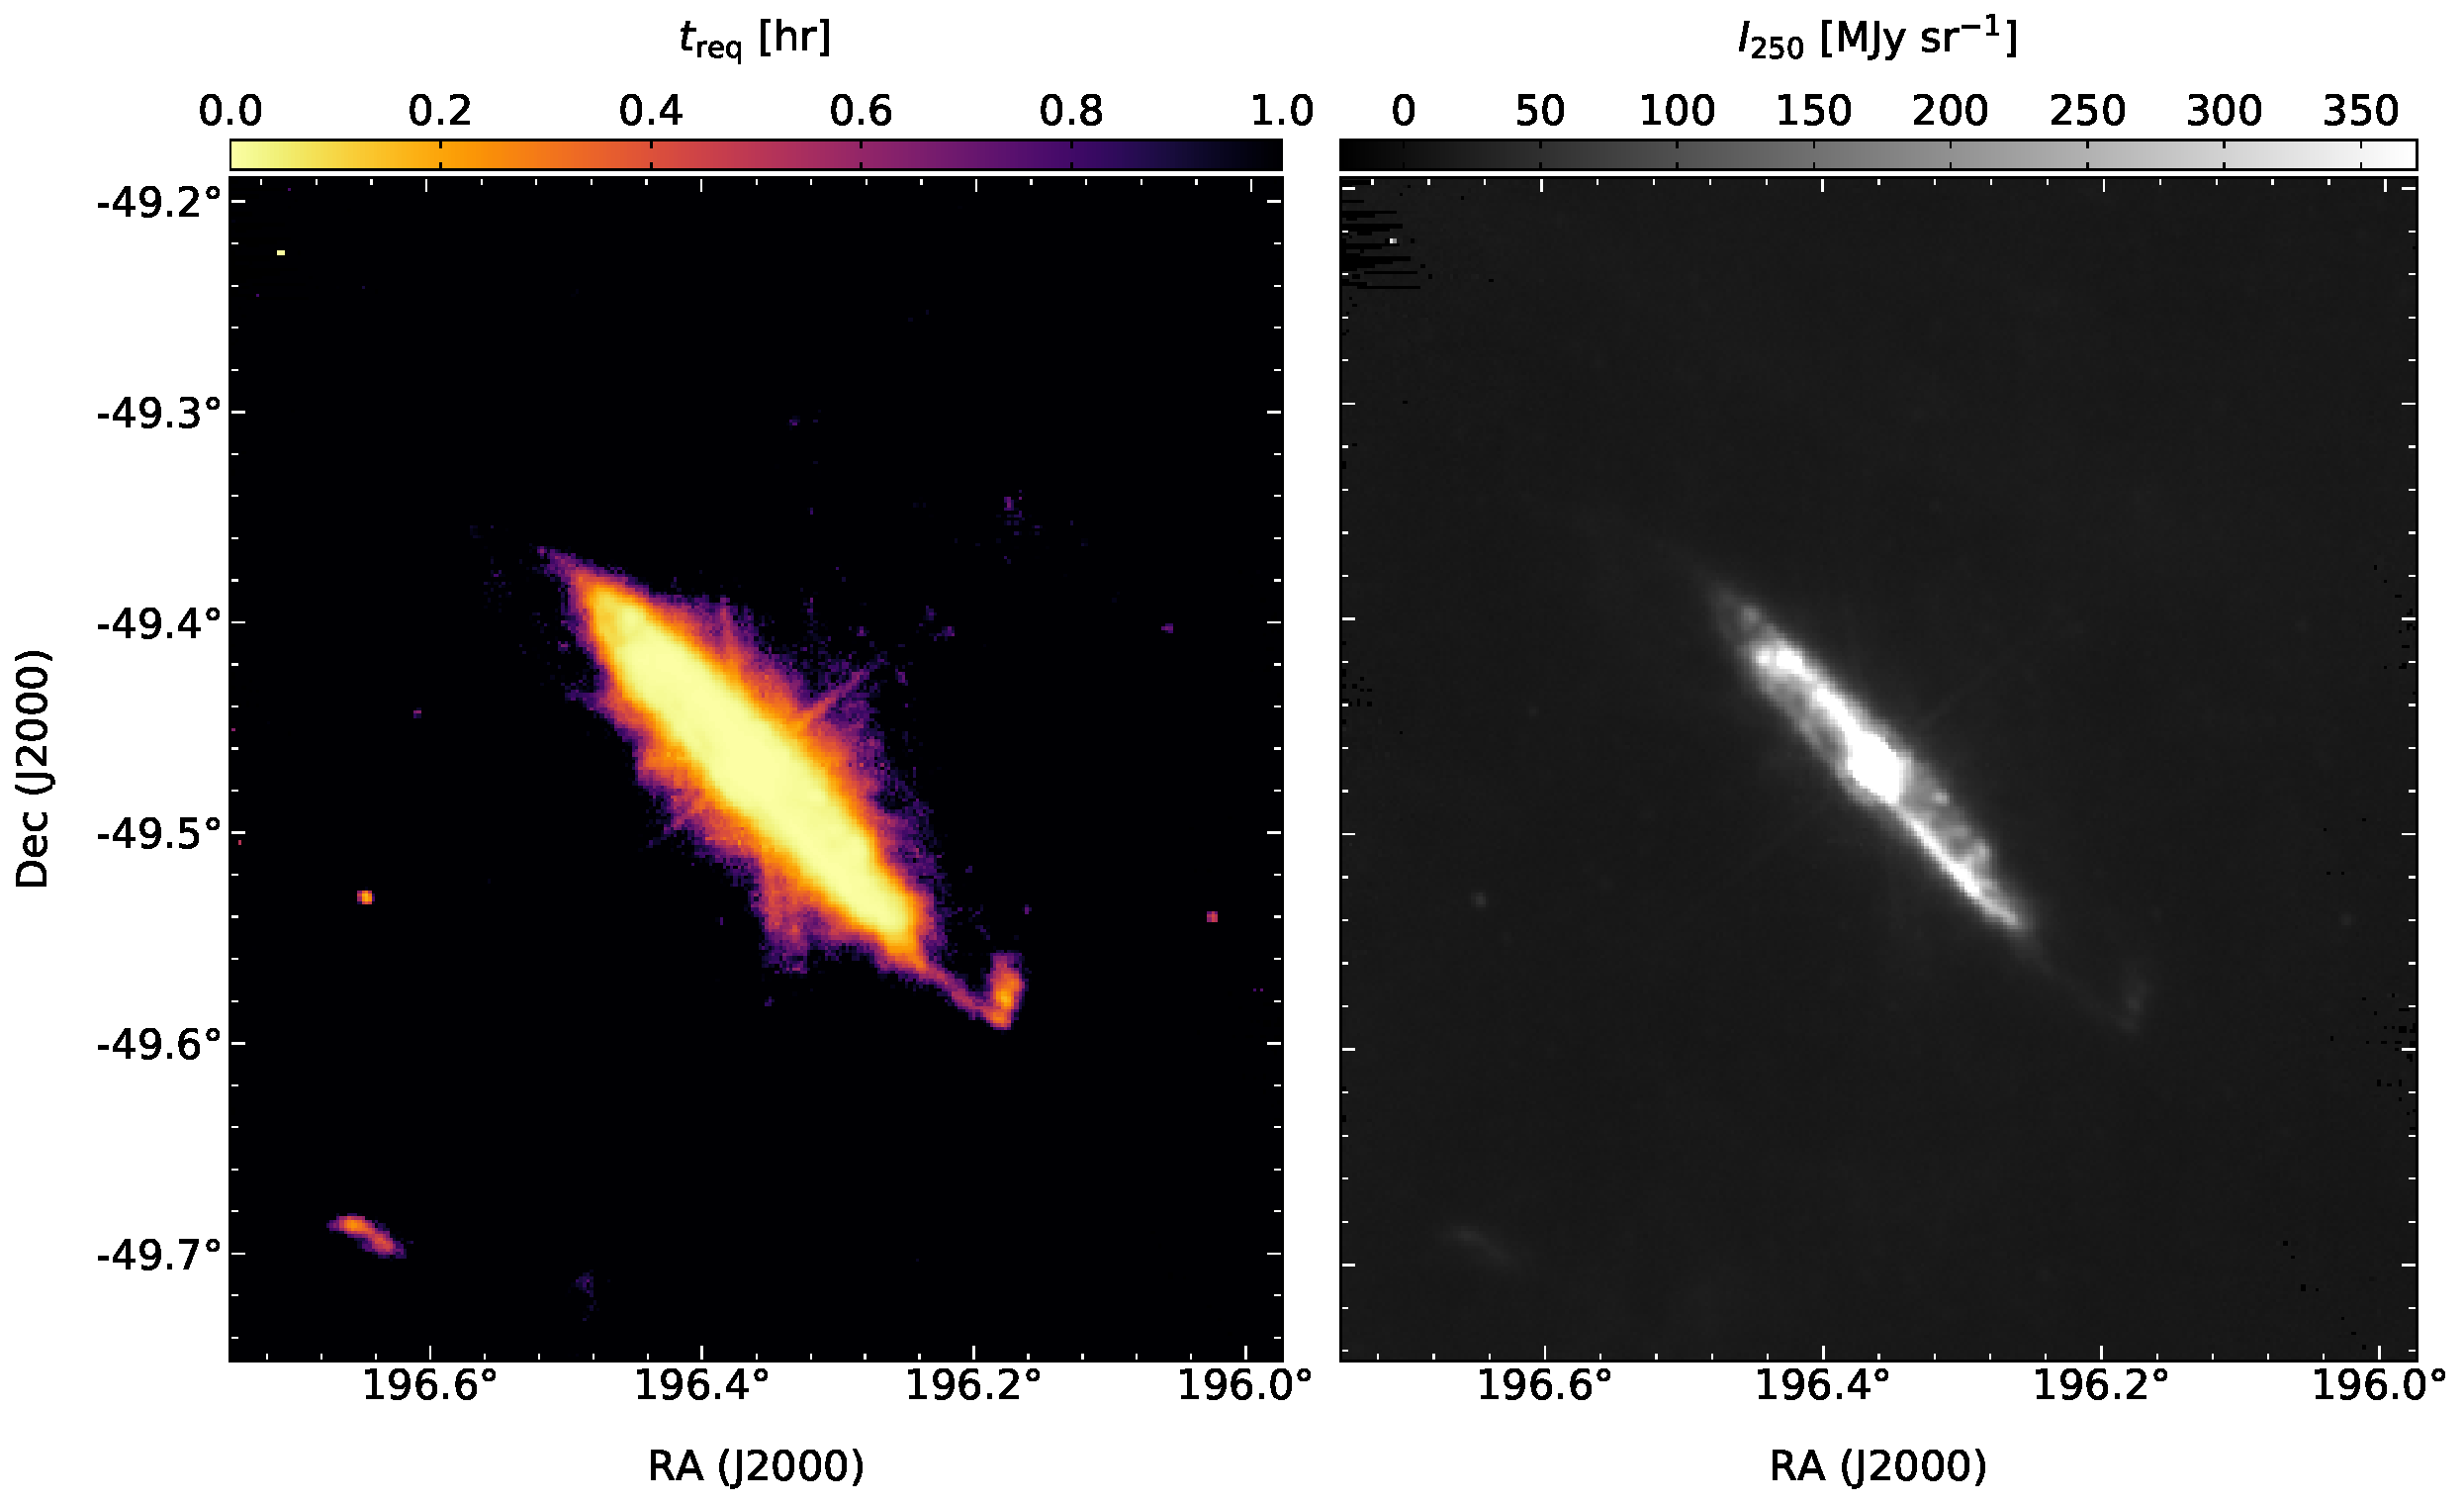
\includegraphics[width=\textwidth]{figures/galaxies/ngc4945}
\caption[NGC 4945 required mapping time.]{NGC~4945: Required mapping time (left) and 250~$\upmu$m intensity, from Herschel SPIRE.}
\label{fig:ngc4945}
\end{figure}

\begin{figure}[!htbp]
\centering
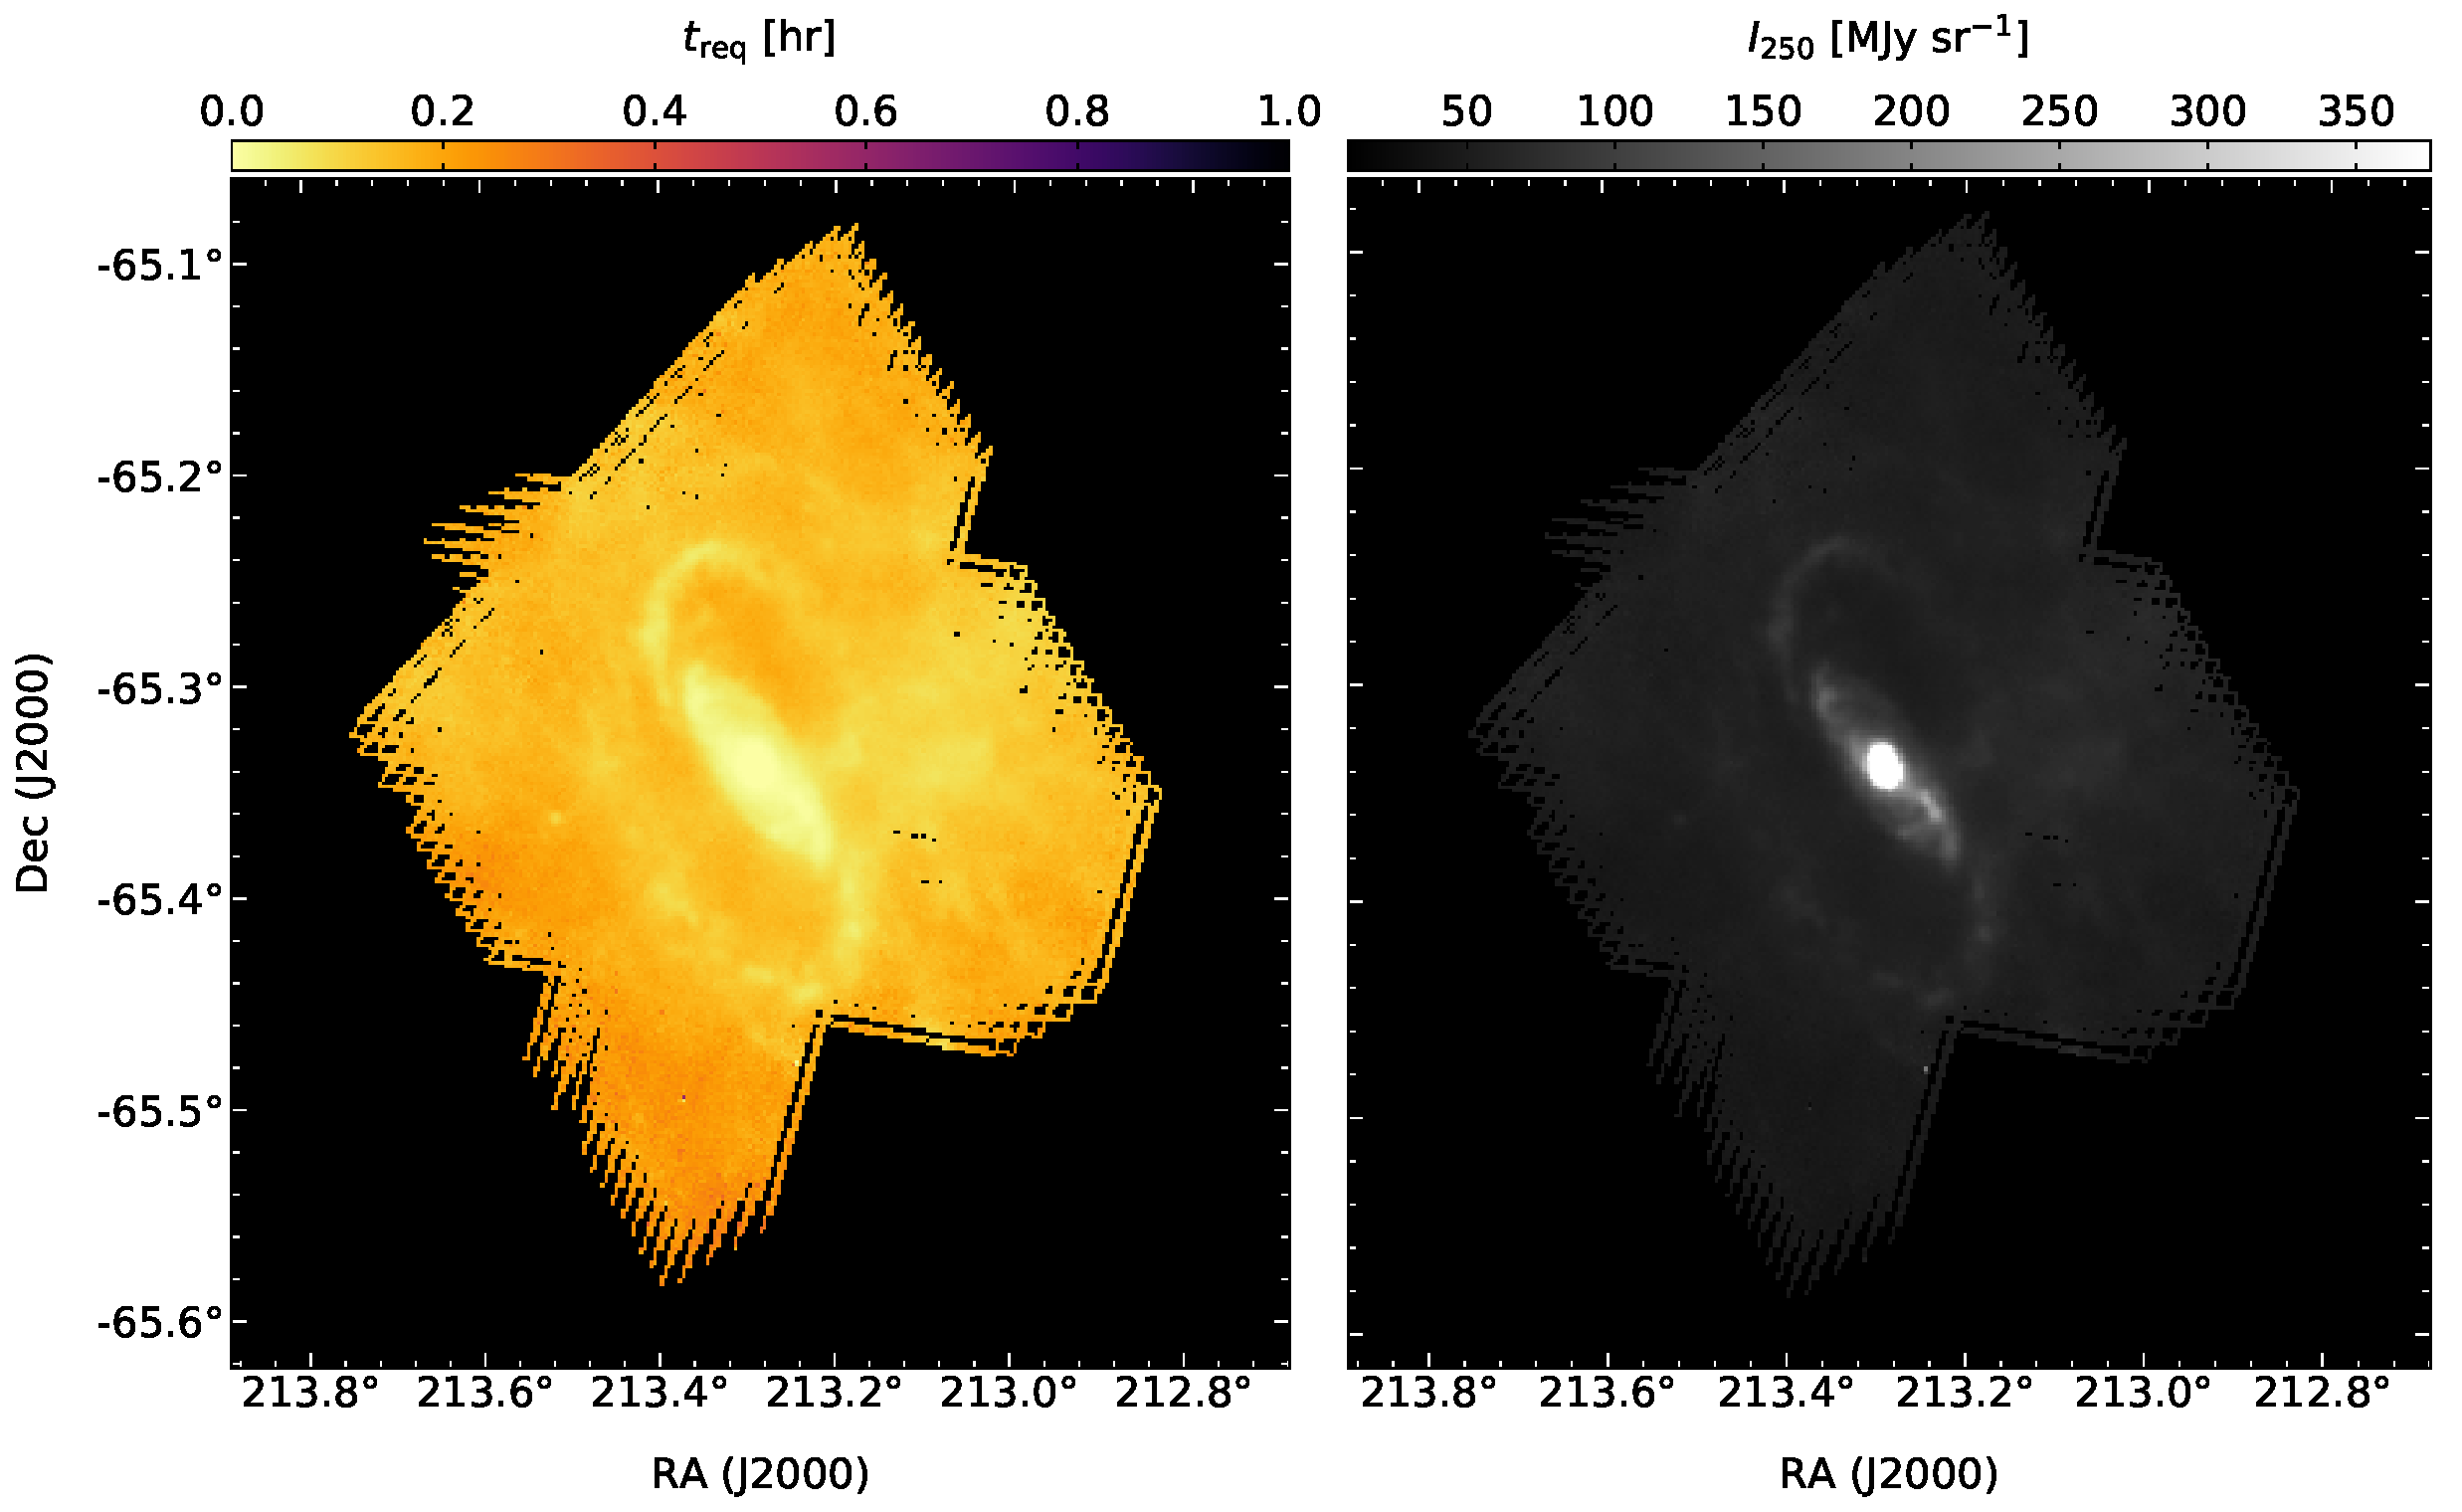
\includegraphics[width=\textwidth]{figures/galaxies/eso9713}
\caption[ESO 97-G13 required mapping time.]{ESO~97-G13: Required mapping time (left) and 250~$\upmu$m intensity, from Herschel SPIRE.}
\label{fig:eso9713}
\end{figure}

\begin{figure}[!htbp]
\centering
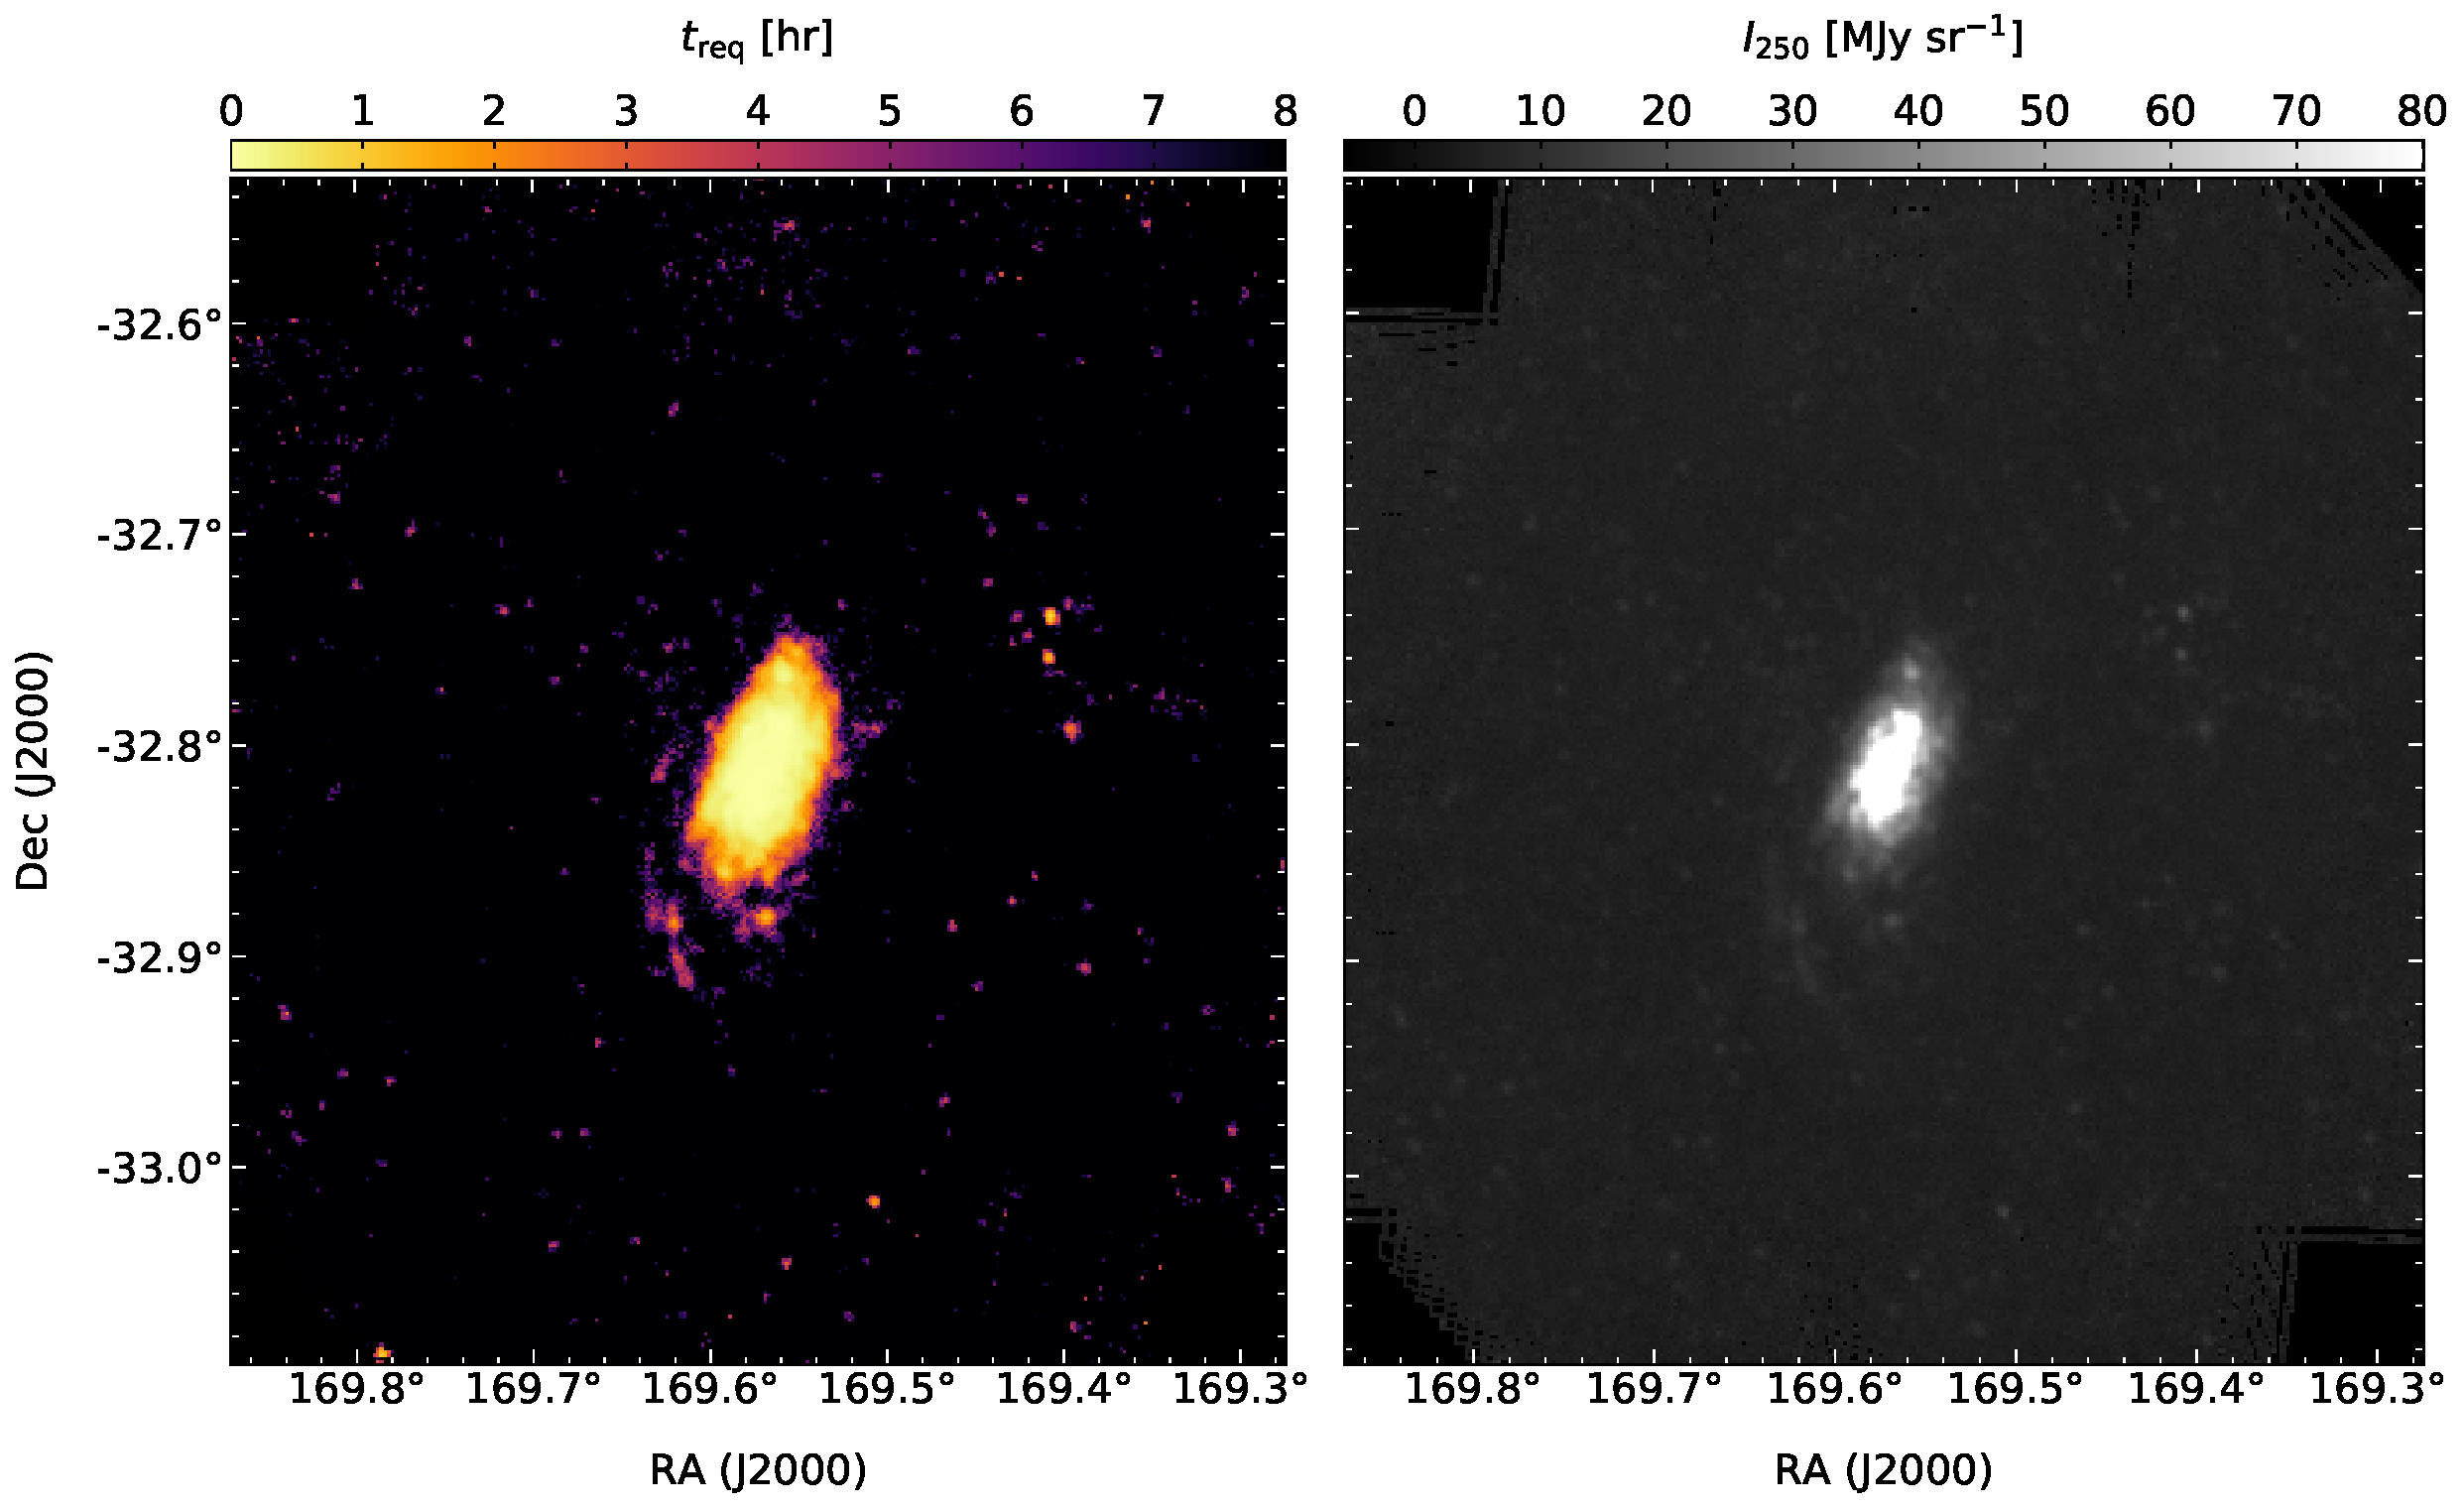
\includegraphics[width=\textwidth]{figures/galaxies/ngc3621}
\caption[NGC 3621 required mapping time.]{NGC~3621: Required mapping time (left) and 250~$\upmu$m intensity, from Herschel SPIRE.}
\label{fig:ngc3621}
\end{figure}

\begin{figure}[!htbp]
\centering
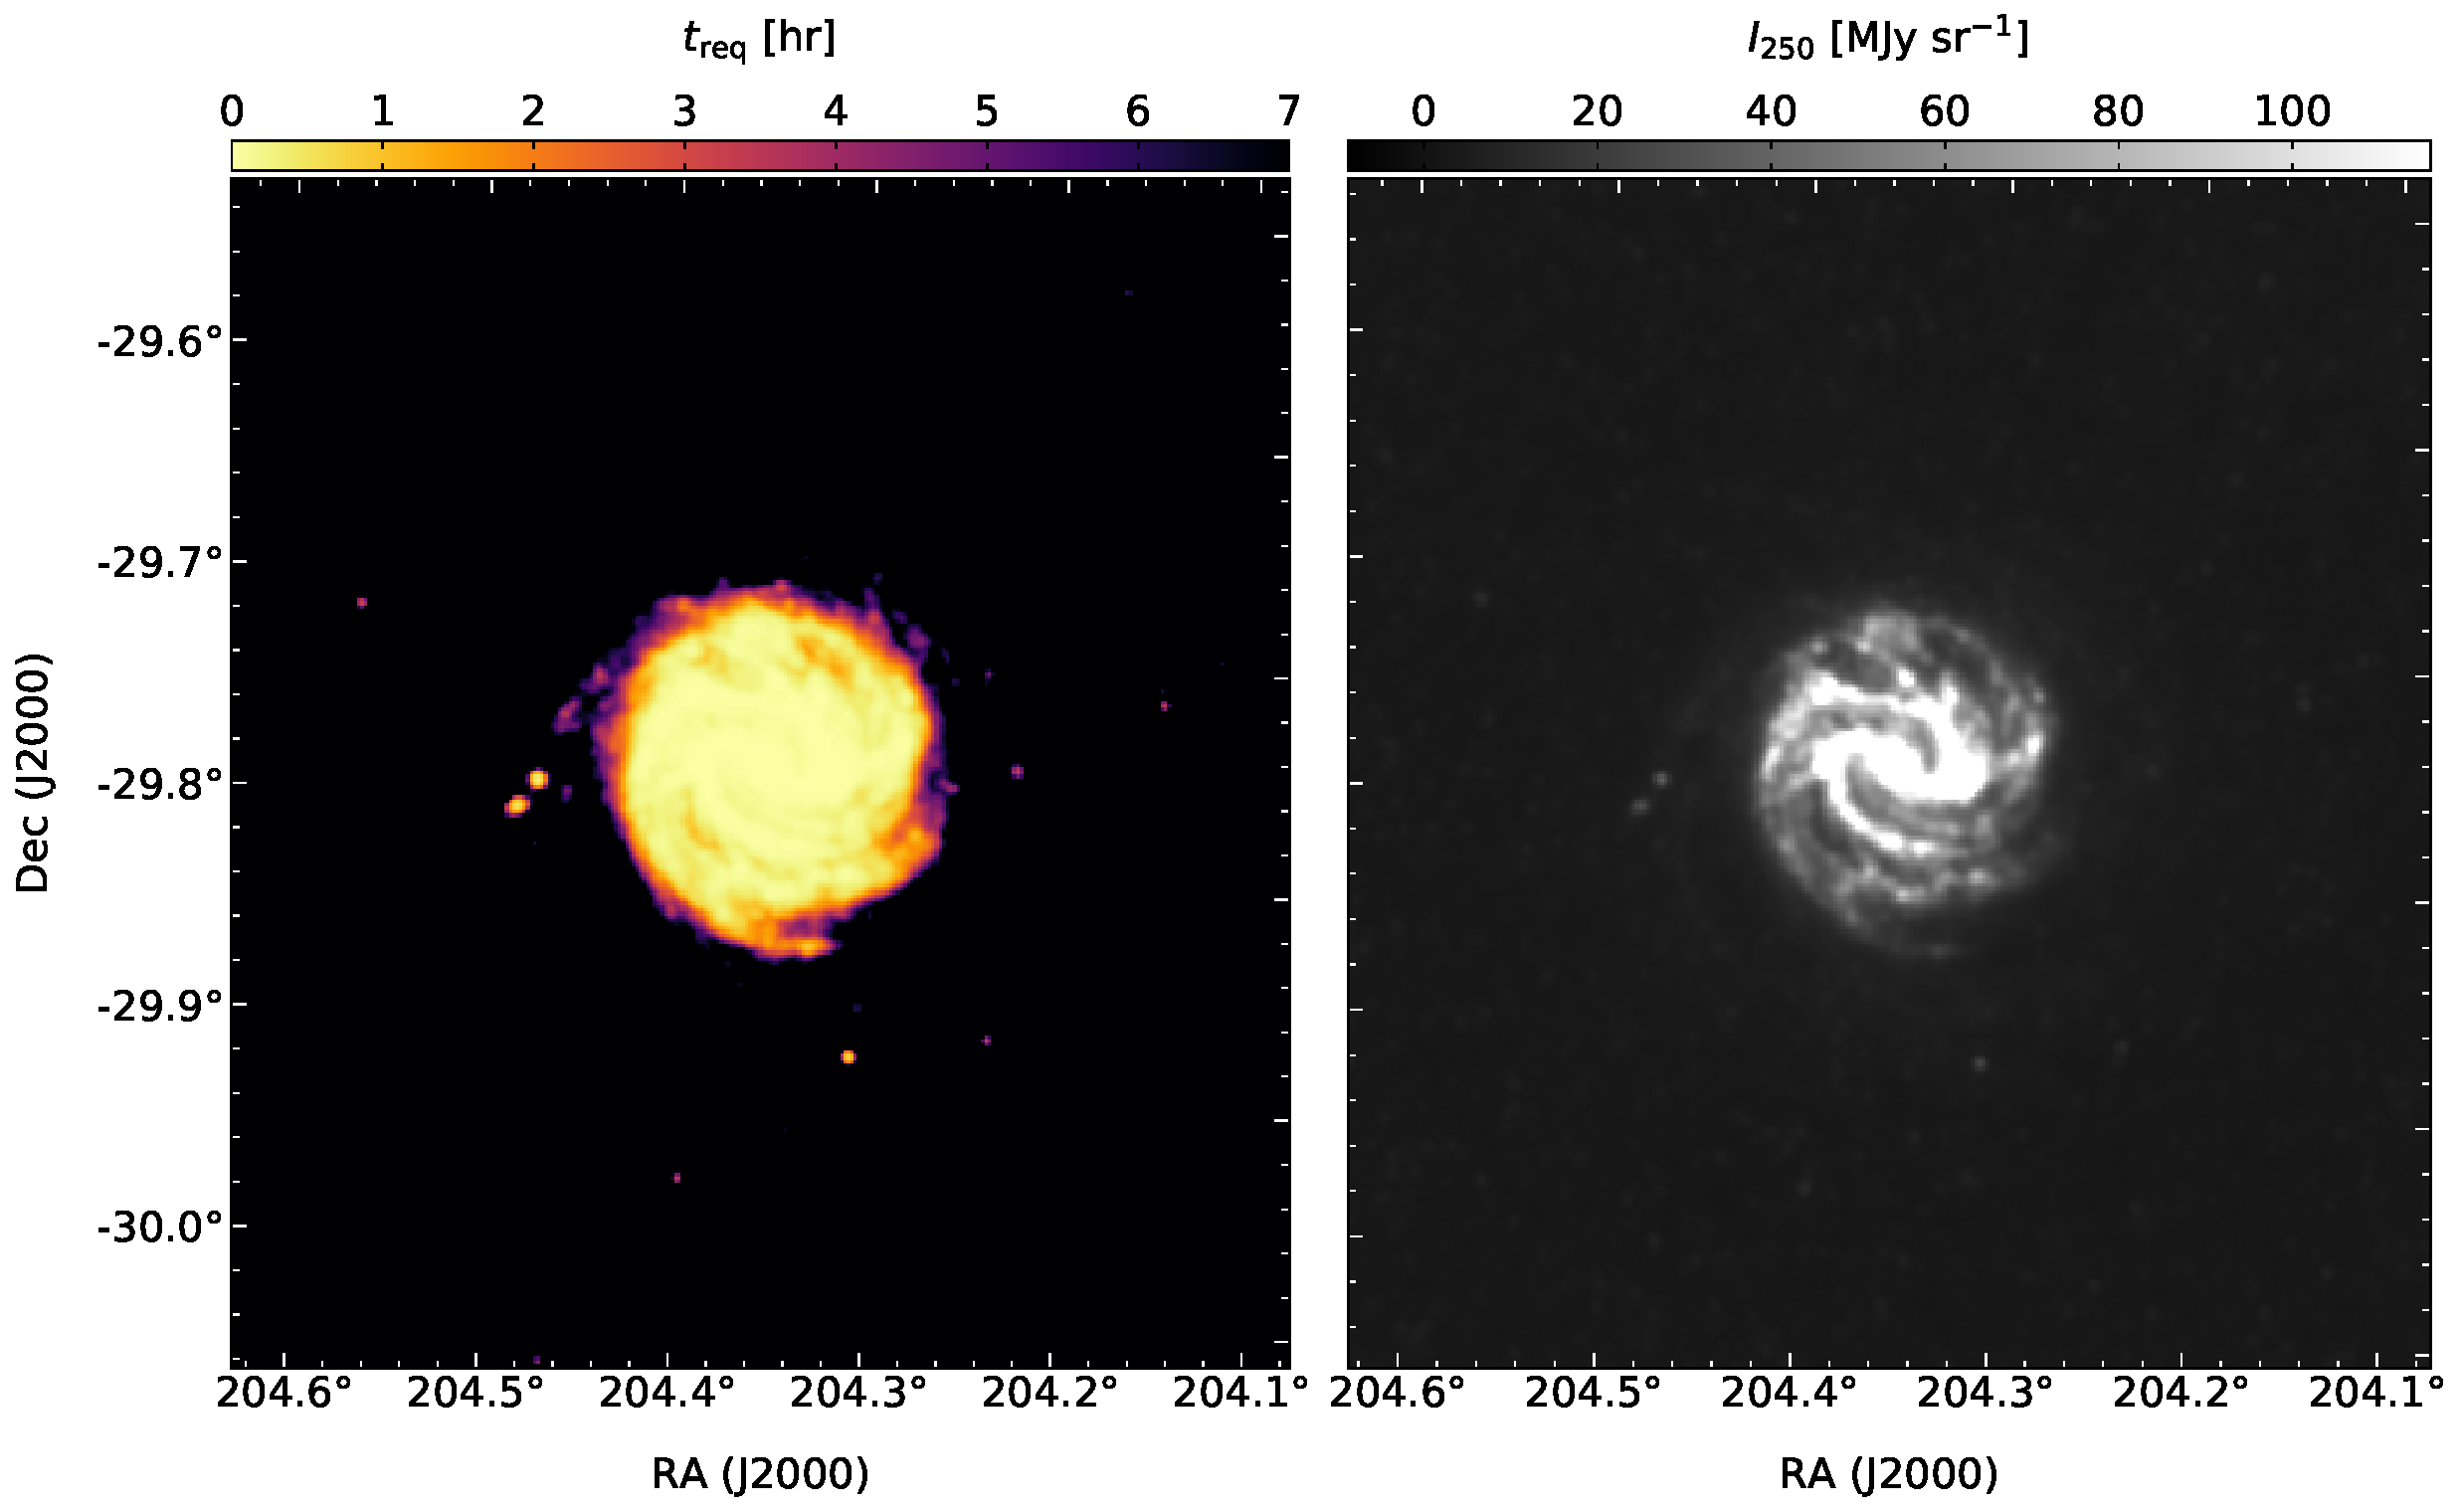
\includegraphics[width=\textwidth]{figures/galaxies/m83}
\caption[M83 required mapping time.]{M83: Required mapping time (left) and 250~$\upmu$m intensity, from Herschel SPIRE.}
\label{fig:m83}
\end{figure}

\begin{figure}[!htbp]
\centering
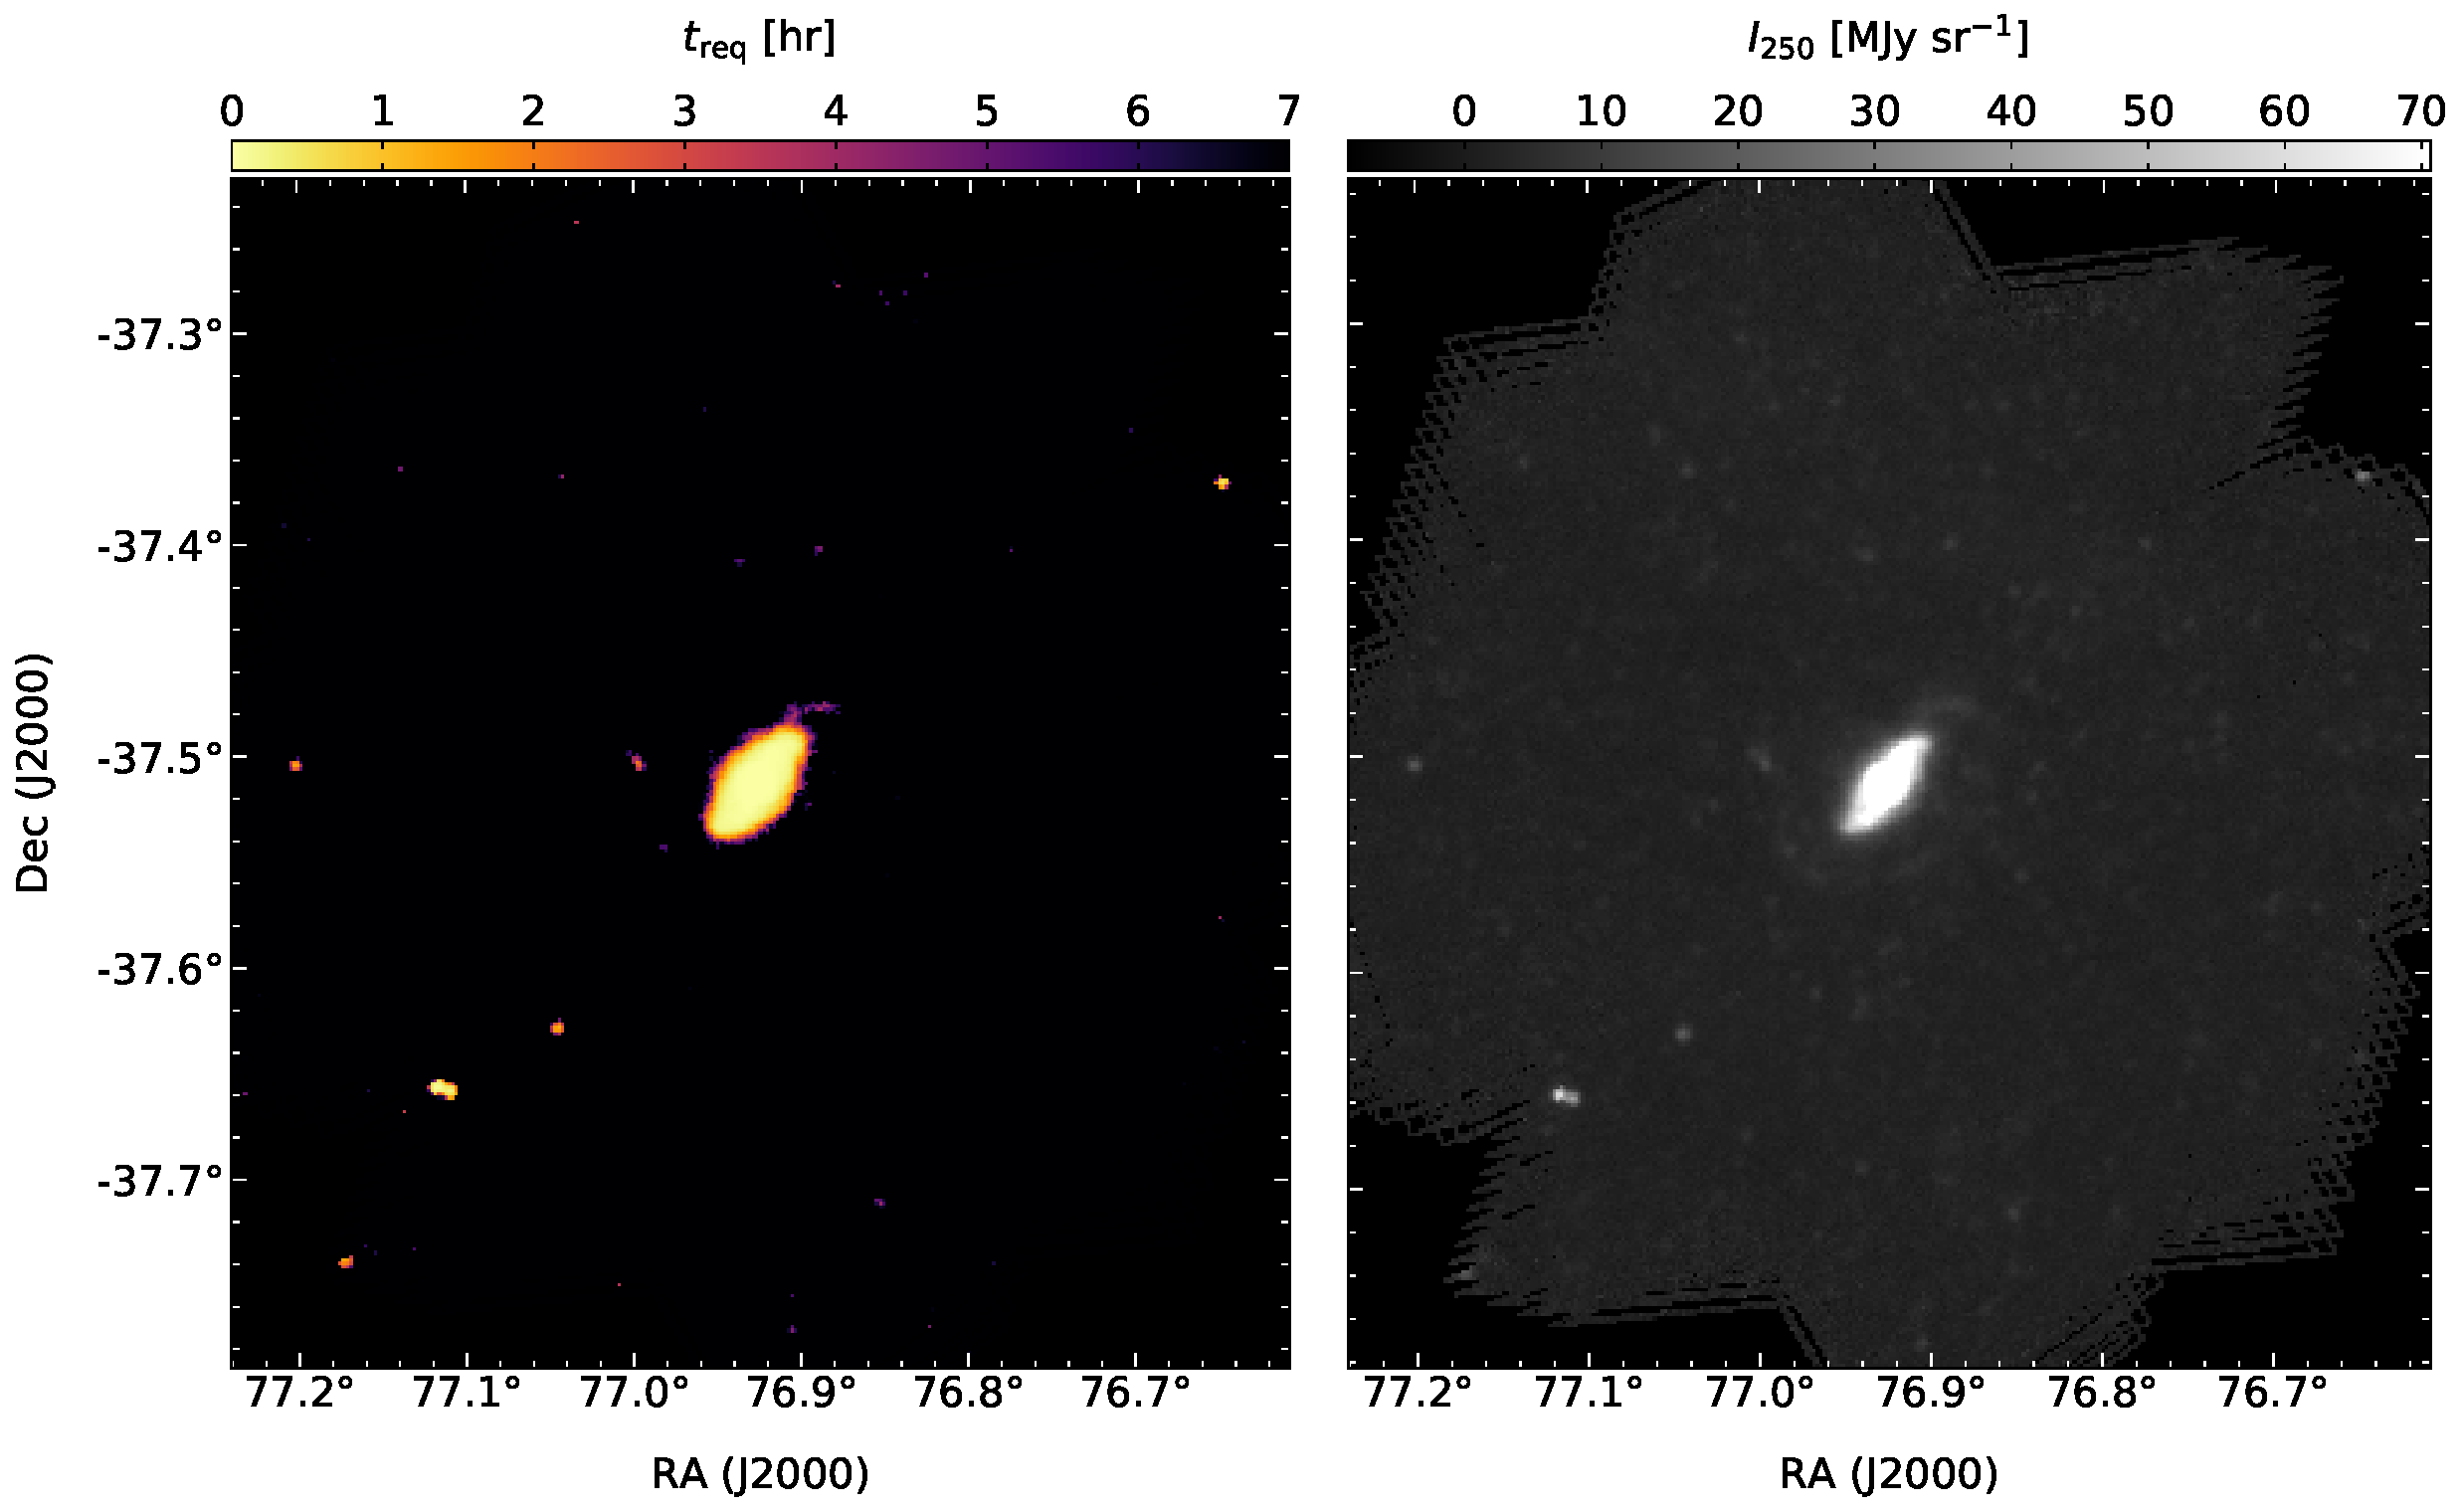
\includegraphics[width=\textwidth]{figures/galaxies/ngc1808}
\caption[NGC 1808 required mapping time.]{NGC 1808: Required mapping time (left) and 250~$\upmu$m intensity, from Herschel SPIRE.}
\label{fig:ngc1808}
\end{figure}
